\section{Results}

%How can I assess the quality of my Results section? To make a self-assessment of your Results section, you can ask yourself the following questions.
%    * Have I expressed myself as clear as possible, so the contribution of my results give stands out for the referees and readers?
%    * Have I limited myself to only reporting the key result or trends each figure and table conveys, rather than reiterating each value?
%    * Have I avoided drawing conclusions? (this is only tr,ue when the Results is an independent section)
%    * Have I chosen the best format to present my data (e.g. figure or table)? Have I ensured there is no redundancy between the figures and tables?
%    * Have I ensured my tables of results are comprehensive in the sense that they do not exclusively include points which prove my point?
%    * Have I mentioned only what my readers specifically need to know and what I will subsequently refer to in the Discussion?
%    * Have I mentioned any parts of my methodology (e.g. selection and sampling procedures) which could have affected my results?
%    * Have I used tenses correctly? past simple for your findings (in the passive form), present simply (descriptions of established scientific fact)


In this section, we present and discuss the review results. Firstly, we present an overview of the selected studies. Secondly, we demonstrate the review findings related to each research question. During the discussion, we also provide related works to support and justify the findings.

\subsection{Overview}

In this study, 26 of the previously selected articles papers were identified in the field of Machine Learning techniques for code smell identification, the selected papers table can be visualized on Annex \ref{app:slrArticles}. The identified papers were published in the period of 1999 to 2016.  Regarding the study type, they have adopted experimentation as methodology. In concern of publication type, there are slightly more conference papers (63\%) than journal papers (37\%).  Only five publications were represented by more than one publication venue: Annual Conference on Genetic and Evolutionary Computation; International Conference on Software Engineering;Journal of Systems and Software; Expert Systems with Applications; Journal of Software: Evolution and Process. These publications represented almost half of the selected papers as shown in Table \ref{tab:papersByPublication}.

\begin{table}[hbt]
\centering
\caption{Papers by publication}
\label{tab:papersByPublication}
\begin{tabular}{ll}
\hline
Publication &                                               \# of studies\\ \hline
Annual Conference on Genetic and Evolutionary Computation &     3   \\
International Conference on Software Engineering &              3   \\
Journal of Systems and Software &                               3   \\
Expert Systems with Applications &                              2   \\
Journal of Software: Evolution and Process &                    2   \\
Others &                                                        13  \\ \hline
\end{tabular}
\end{table}

The topmost of the selected papers are recent, the papers published in the last 2 years respond for above 50\% of the selected papers as can be observed in Figure \ref{fig:papersByYear}. Confirming the observation of previous studies~\citep{rasool2015review, fontana2016comparing} which shows a growing interest in Machine Learning techniques for code smell identification.

\begin{figure}[hbt] 
    \centering
	\caption{Papers by year}
	\label{fig:papersByYear}
	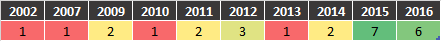
\includegraphics[]{imagens/papersByYear.png}
\end{figure}

The selected papers used Java as its code source language. From the 26 selected, 23 used open source projects, while only 3 used private data source. As displayed on Figure \ref{fig:StudiesBySourceDisponibility}.

\begin{figure}[hbt] 
    \centering
	\caption{Data source by source code license}
	\label{fig:StudiesBySourceDisponibility}
	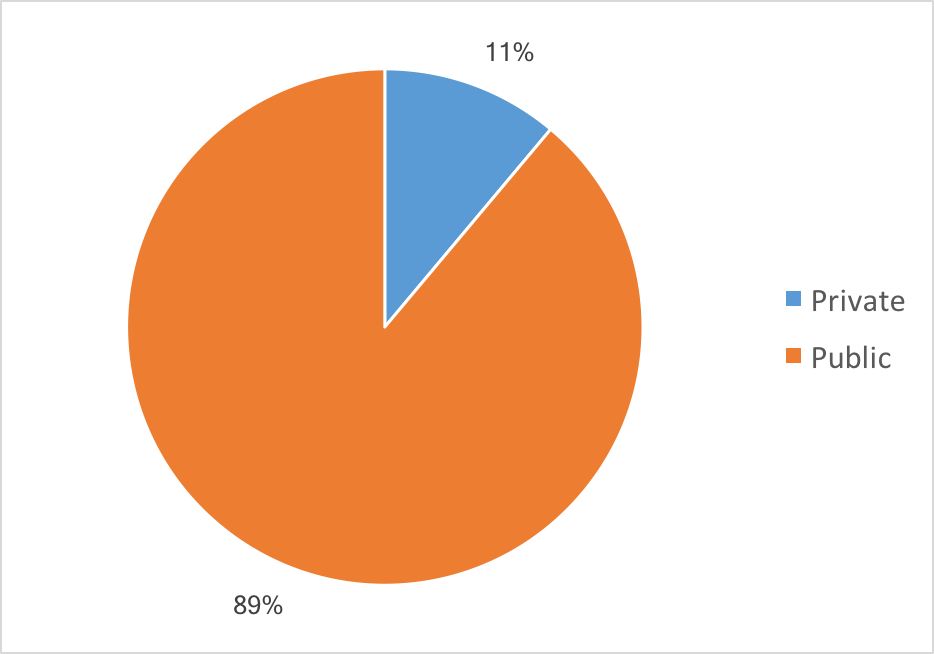
\includegraphics[width=0.6\textwidth]{imagens/StudiesBySourceDisponibility.png}
\end{figure}

The 24 studies that used open source code, used 65 projects. From which we can highlight: Xerces with 7\%, JHotDraw - 6\%, Eclipse Core - 6\%, ArgoUML - 5\%, JFreeChart - 3\% and GanttProject - 3\%. As detailed by Figure \ref{fig:StudiesByDataSource}.

\begin{figure}[hbt] 
    \centering
	\caption{Used open source projects}
	\label{fig:StudiesByDataSource}
	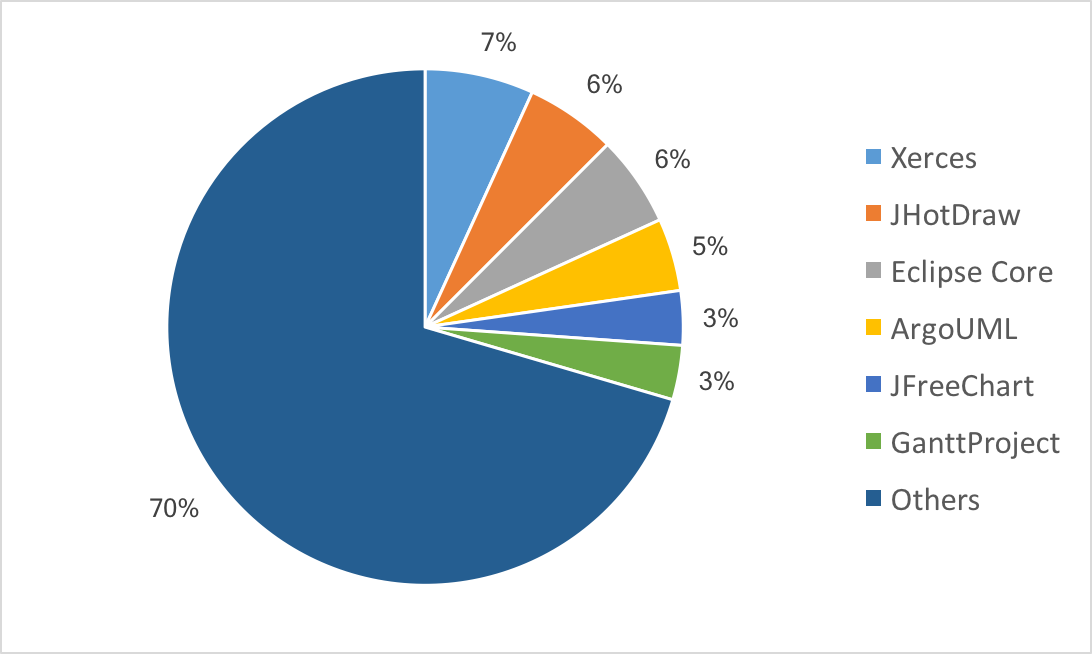
\includegraphics[width=0.6\textwidth]{imagens/StudiesByDataSource.png}
\end{figure}

\subsection{Which code smells are addressed when using Machine Learning techniques for the identification?}

In this study, we used the 22 code smells defined by~\cite{fowler1999refactoring} as base for our classification, we also used 3 of the anti-patterns defined by~\citep{brown1998antipatterns} related to code related design flaws. There is also the "others" classification meant to capture smells defined by other authors and code-flaws not related to a specific smell, since the authors aim at code metrics optimization instead of a specific smell.

Comparing the studied code-related design flaws using machine learning, the ones with higher appearance were Feature Envy (FE) smell and BLOBs both  studied by 5 papers, followed by Long Methods (LM) that appeared in 4. While Comments (COM), Primitive Obsession (PO), Refused Bequest, Alternative Classes with Different Interfaces (ACDI) and Incomplete Library Class (ILC) were not addressed by any of the studied papers. The distribution of the smells is show in Figure \ref{fig:papersBySmell}. Except for the duplicated code which is usually the mainly studied smell, the other smells are coherent with the ones identified by~\cite{zhang2011code} in his review. The others category, composed mainly by optimization in the code metrics appeared 8 times, using alternatives to the traditional code smells.

\begin{figure}[!ht] 
    \centering
	\caption{Papers by Code Smell}
	\label{fig:papersBySmell}
	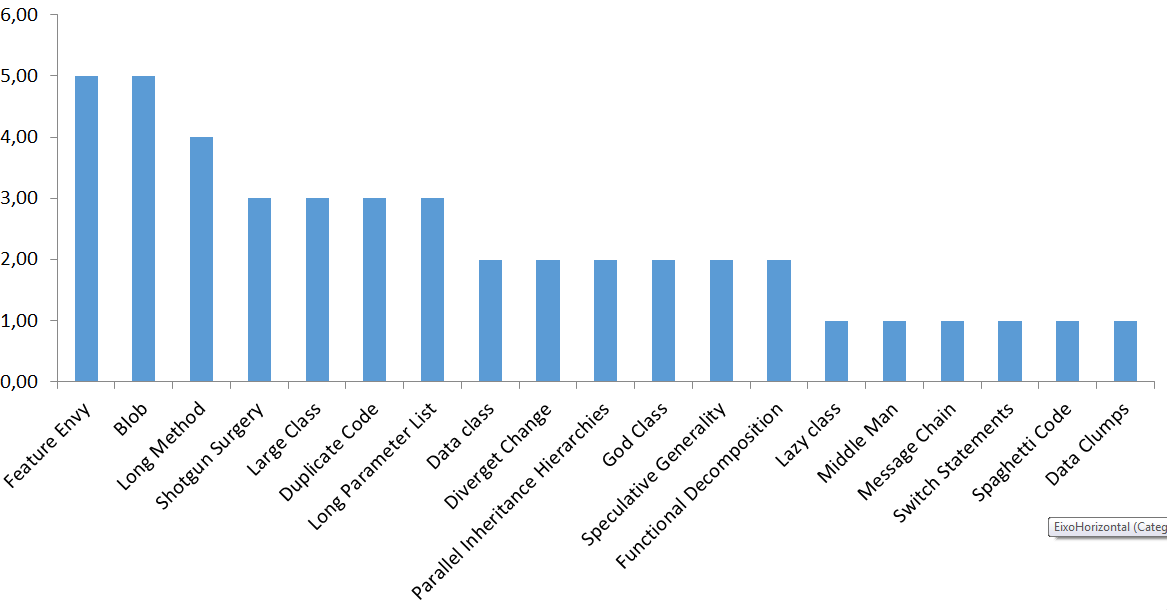
\includegraphics[width=0.95\textwidth]{imagens/papersBySmell.png}
\end{figure}

When grouping by the classification defined by~\cite{mantyla2003bad} it is possible to observe that the main focus regarding the addressed type of smell are the Bloaters representing 35\% of the studied smells. Follows to this: The Dispensables (15\%); The Object-Orientation Abusers (9\%); The Change Preventers (9\%); The Couplers (9\%); The Encapsulators (4\%). The other code smells, mainly represented by metrics-based representations, represent 17\%. As detailed on Figure \ref{fig:papersBySmellType}.

\begin{figure}[!ht] 
    \centering
	\caption{Papers by Code Smell Type}
	\label{fig:papersBySmellType}
	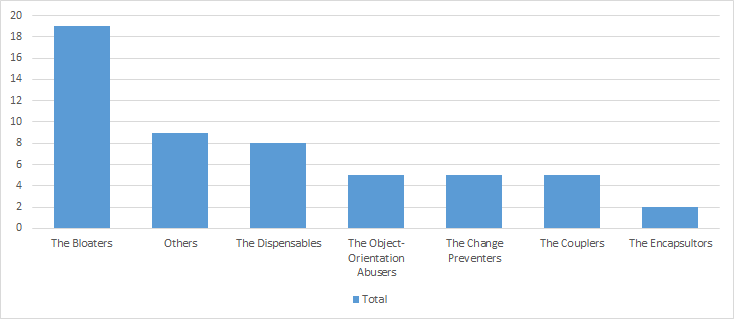
\includegraphics[width=0.95\textwidth]{imagens/papersBySmellType.png}
\end{figure}

When studying the smells usually studied together, one of the strongest co-occurrence is between BLOB, Spaghetti Code (SC) and Functional Decomposition (FD), one of the main reasons is that, apart from the others, they were not defined by~\cite{fowler1999refactoring}, but by~\cite{brown1998antipatterns}. Duplicated code also had a strong co-occurrence with Data Clumps (DCP) and Shotgun Surgery (SS), but the reciprocal was not true, one of the explanations is that Duplicated Code (DUC) is usually studied alone. Feature Envy also receives highlight when comparing smells usually studied together, it is studied together with part of the smells. Others that deserve mention are Long Parameter List (LPL), Long Methods (LM) and Large Class (LC). The co-occurrence matrix is shown in details in Figure \ref{fig:smellsCoOccurrence}.

\begin{figure}[!ht] 
    \centering
	\caption{Number of times a smell was studied with another by paper}
	\label{fig:smellsCoOccurrence}
	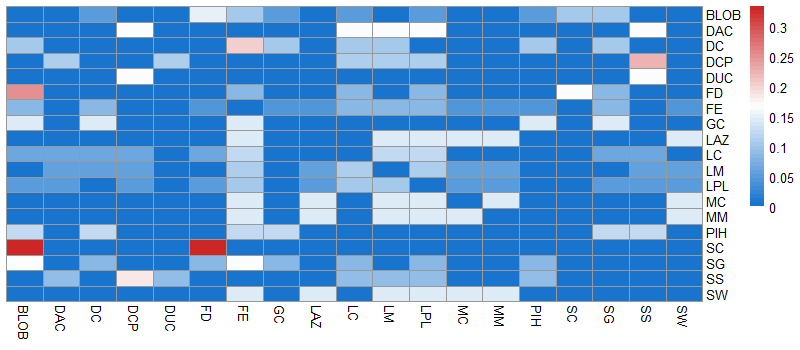
\includegraphics[width=0.95\textwidth]{imagens/smellsCoOcurrenceHM.png}
\end{figure}

\subsection{Which Machine Learning techniques are used when identifying code smells?}

The leading technique in the analyzed papers was the Genetic Algorithm which appeared 8 times, this technique is used mainly in search-based techniques, and focuses on optimizing one or more metric by mutating and evolving the code. Followed by Naive Bayes Classifiers that appeared 4 times. While a approaches such as: Linear discriminant analysis (LDA); Decision Tree; Support; Vector Machine (SVM); Directed Acyclic Graph (DAG); Text-Based - appeared only once. The distribution can be visualized in Figure \ref{fig:papersByMLTechnique}.

\begin{figure}[!ht] 
    \centering
	\caption{Papers by Machine Learning Technique}
	\label{fig:papersByMLTechnique}
	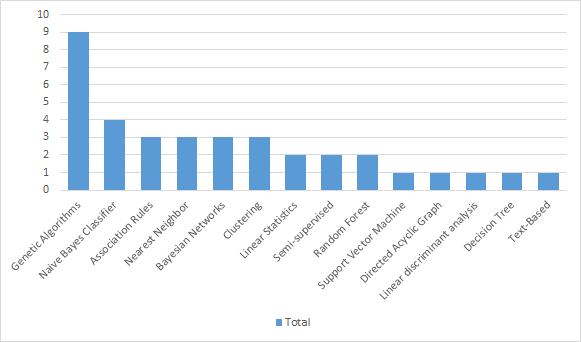
\includegraphics[width=0.95\textwidth]{imagens/papersByMLTechnique.png}
\end{figure}

Regarding the kind of technique used the supervised techniques were the main one, being used in 32 tests (88\%); Semi supervised and unsupervised techniques appeared only 2 (6\%) times which. The results was expected since supervised tests are the greatly used in researches~\citep{kotsiantis2007supervised}.

\subsection{Which Machine Learning techniques are most used for each kind of code smell?}

The smells addressed by the techniques were coherent with the smells that appeared in the related papers, showing a high level of redundancy. The smell focused by the majority of the techniques was Feature Envy (FE), which was aimed by 9 techniques (64\%). Followed by Long Method (LM) with 8 techniques (57\%) and Long Parameter List (LPL) with 7 (50\%). From the smells targeted by the studied papers, the ones covered by less techniques were Speculative Generality (SG), Spaghetti Code (SC), Data Class (DAC),  God Class (GC), Parallel Inheritance (PIH) and Data Clumps (DCP) with 2 techniques each (14\%).

From a Machine Learning technique perspective, the Association Rules techniques was the technique with broader usage, covering 13 smells (59\% of them), followed by linear statistics with 11 smells (50\%), Naive Bayes and Random Forest with 9 smells (43\%). While Text-Based and Linear Discriminant Analysis with 1 smell (5\%) are in the lower half.


When comparing the number of times a code smell was addressed by a given technique, there was no clear relationship. Although the smells coverage is higher for a given technique, e. g., Feature Envy (FE) and Bayesian Network, it does not displays a clear pattern. The relation between smells and techniques can be visualized in Figure \ref{fig:smellsXMLTechniques}

\begin{figure}[!ht] 
    \centering
	\caption{Number of times a smell was studied with another by technique}
	\label{fig:smellsXMLTechniques}
	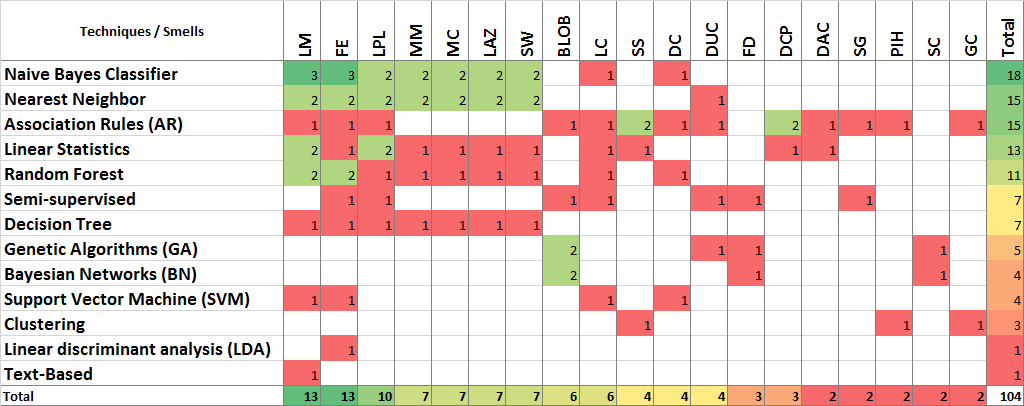
\includegraphics[width=0.95\textwidth]{imagens/smellsXMLTechniques.png}
\end{figure}

However when comparing the smells by type, we found out that the Association Rules technique with a relevant focus on the Change Preventers type of smell, as the graph nature of technique allows it to analyse the relationship between methods and classes. The other smell types followed the same patterns presented when comparing the coverage by papers and the classifiers the same pattern as discussed previously.

\begin{figure}[!ht] 
    \centering
	\caption{Code Smell type by Machine Learning technique}
	\label{fig:smellsTypeXMLTechniques}
	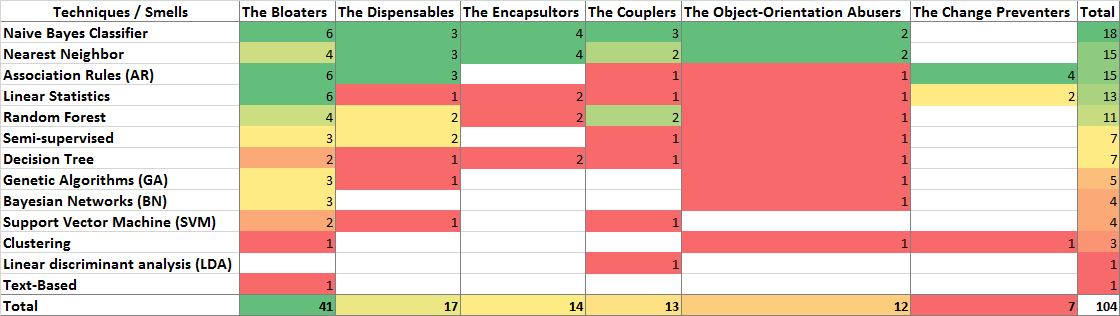
\includegraphics[width=0.95\textwidth]{imagens/smellsTypeXMLTechniques.png}
\end{figure}

When we analyse the co-occurrence matrix of code smells by Machine Learning technique it displays a similar pattern to the one presented when analyzing the code smells co-occurrence by papers, as demonstrated on Figure \ref{fig:smellsXMLTechniquesCoOcurrence}. With the~\cite{brown1998antipatterns} code anti-patterns presenting a high co-occurrence, and the Long Method (LM), Feature Envy (FE) and Long Parameter List (LPL) presenting a more heterogeneous application. This can be explained by the fact that, in general, the studied papers focuses on only one technique.

\begin{figure}[!ht] 
    \centering
	\caption{Code smells co-occurrence by Machine Learning technique}
	\label{fig:smellsXMLTechniquesCoOcurrence}
	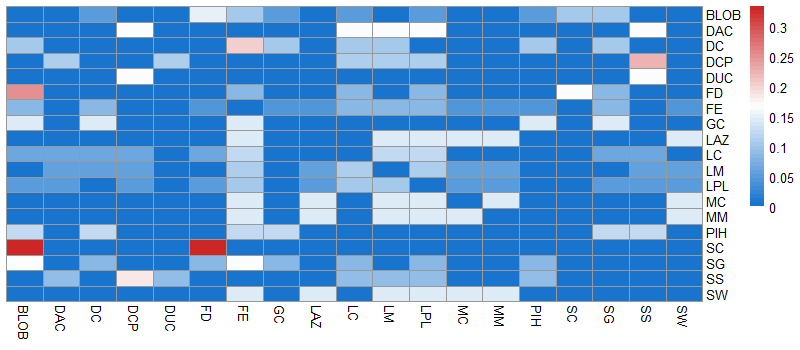
\includegraphics[width=0.95\textwidth]{imagens/techniqueXSmellOcurrenceHM.png}
\end{figure}

\subsection{Which Machine Learning techniques performs better for each smell?}

One hardship we found when comparing the techniques performance is the lack of standardized data. 14 out of the 26 papers provided performance info. From those, 13 provided precision data, 12 provided recall values and only 6 provided us with F-measures. So, although these aspects are complementary, we had to analyze them separately. To have comparable parameters we also selected only the papers that used the same baseline as the majority of the articles, in this case a manual annotation of the code smells.

In terms of f-measure the best average performance was provided the Random Forest technique, followed by Decision Tree, Semi-supervised and Naive Bayes Classifier techniques. While Association Rules and Support Vector Machine, had a heterogeneous performance, presenting a high variation. Compared to them the textual analysis had the worst performance between the studied practices, as demonstrated by Figure \ref{fig:fmeasureByTechniques}.

\begin{figure}[!ht] 
    \centering
	\caption{Machine Learning techniques F-measure Box-plot}
	\label{fig:fmeasureByTechniques}
	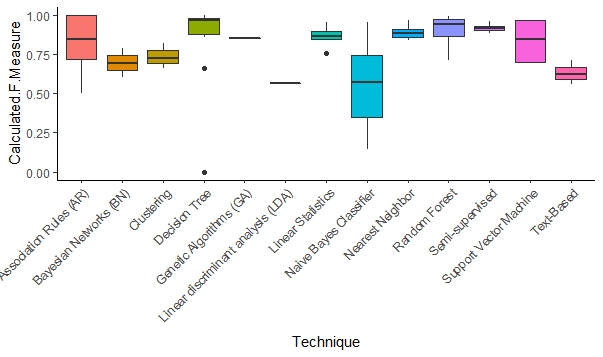
\includegraphics[width=0.9\textwidth]{imagens/fmeasureByTechniques.png}
\end{figure}

When comparing the results by f-measure as demonstrated by Figure \ref{fig:techniqueXSmellFMeasure}, it is possible to notice that the Association Rules technique performed above the others for Data Clumps (DCP) and Speculative Generality (SG) smells, the ones which only this technique informed it. But performs poorly for Duplicated Code (DUC) and Feature Envy (FE), when compared to the other techniques. For the other smells, there was no outstanding technique.

\begin{figure}[!ht] 
    \centering
	\caption{Technique F-Measure by code smell}
	\label{fig:techniqueXSmellFMeasure}
	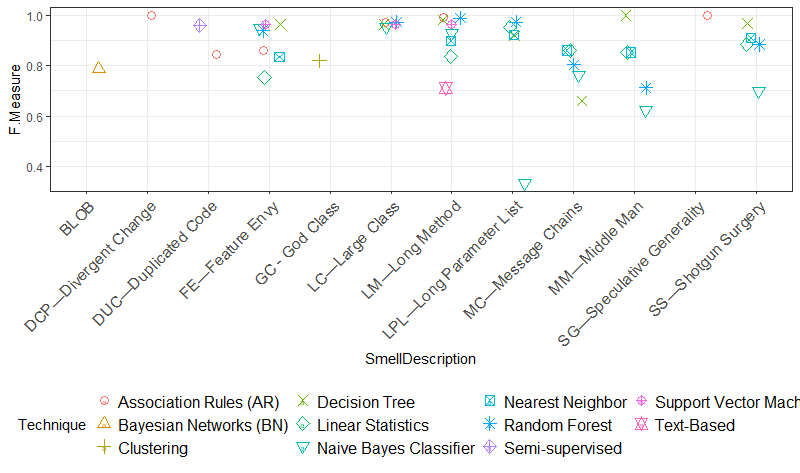
\includegraphics[width=0.95\textwidth]{imagens/TechniqueXSmellFMeasure.png}
\end{figure}

When analysing the techniques by precision, the Linear Discriminant Analysis technique presented the best average performance, followed respectively to its performance by Association Rules, Semi-supervised, Decision Tree, Genetic Algorithm, Linear Statistics, Random Forest and Clustering. In this aspect the worst performing techniques were the Bayes based techniques: Naive Bayes Classifier and Bayesian Networks. The results can be visualized in Figure \ref{fig:precisionByTechniques}.

\begin{figure}[!ht] 
    \centering
	\caption{Machine Learning techniques Precision Box-plot}
	\label{fig:precisionByTechniques}
	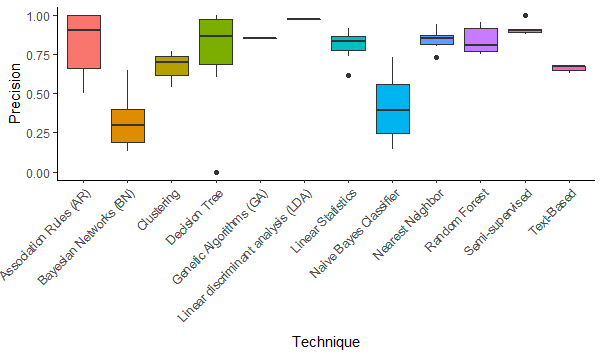
\includegraphics[width=0.9\textwidth]{imagens/precisionByTechniques.png}
\end{figure}

Comparing the techniques by precision, Association Rules, also demonstrated an outstanding performance on Data Clumps (DCP) and Speculative Generality (SG), where it is the only technique used. Semi-supervised techniques had an outstanding performance for Duplicated Code (DUC), Random Forest for FE and Decision Tree for Lazy Class (LZC) and Middle Man (MM) also deserves mention. We had the Bayesian Networks and Naive Bayes Classifiers performing poorly than the other techniques on the smells. Those observations are displayed in Figure \ref{fig:techniqueXSmellPrecision}.

\begin{figure}[!ht] 
    \centering
	\caption{Technique Precision by code smell}
	\label{fig:techniqueXSmellPrecision}
	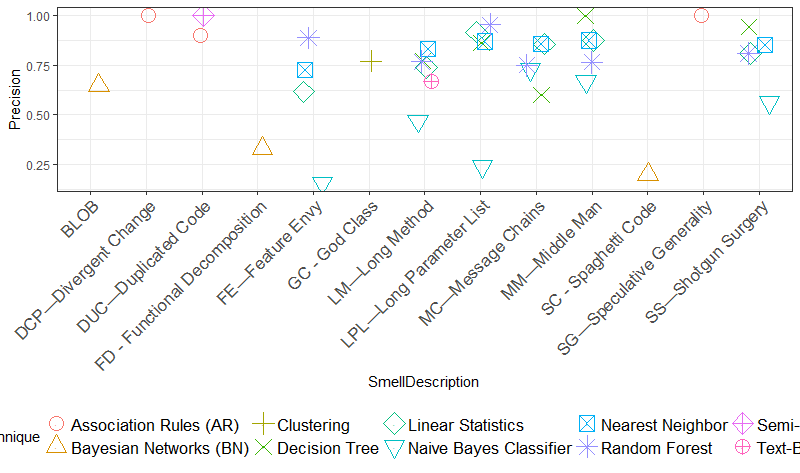
\includegraphics[width=0.95\textwidth]{imagens/TechniqueXSmellPrecision.png}
\end{figure}

When compared by recall, the techniques, in general, performed above 80\%. The best performing techniques under this perspectives were: Bayesian Networks, Decision Tree, Random Forest, Nearest Neighbor, Linear statistics, Semi-supervised, Genetic Algorithm and Clustering. While the worst performing was Naive Bayes classifier, Text-Based and Linear Discriminant Analysis, as displayed by Figure \ref{fig:recallByTechnique}.

\begin{figure}[!ht] 
    \centering
	\caption{Machine Learning techniques recall Box-plot}
	\label{fig:recallByTechnique}
	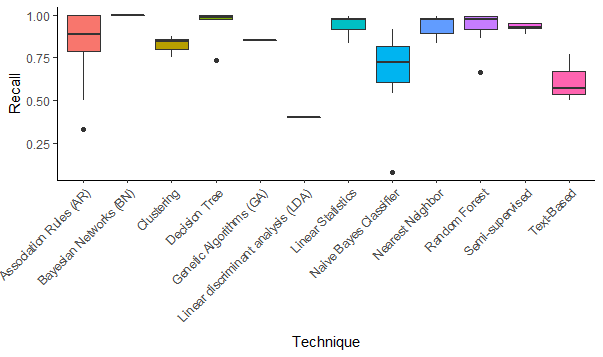
\includegraphics[width=0.9\textwidth]{imagens/recallByTechnique.png}
\end{figure}

Assessing the technique by smells under a Recall perspective as demonstrated in Figure \ref{fig:techniqueXSmellRecall}. As occurred in the previous perspective we have the Naive Bayes classifier performing worst in general, other techniques which displayed a bad performance was Random Forest for Middle Man (MM), Decision Tree for Message Chain (MC) and Text-Based technique for Long Method (LM).

\begin{figure}[!ht] 
    \centering
	\caption{Technique Recall by code smell}
	\label{fig:techniqueXSmellRecall}
	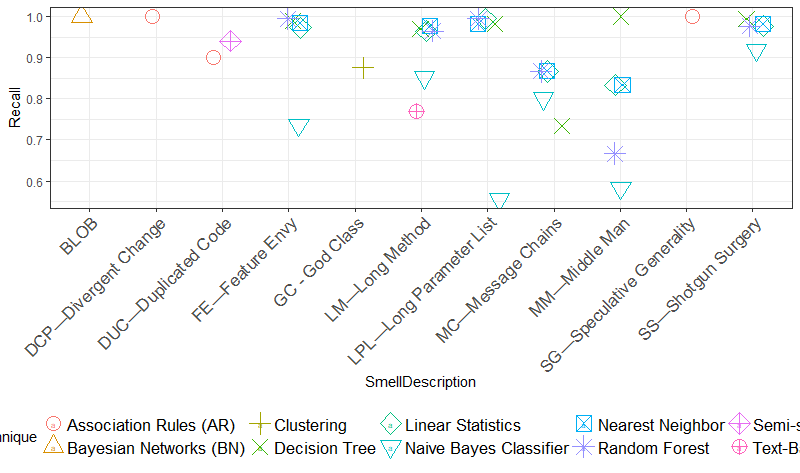
\includegraphics[width=0.95\textwidth]{imagens/TechniqueXSmellRecall.png}
\end{figure}

%%%%%%%%%
\section{Discussion}
\label{sec:discussion}
%%%%%%%%%

This studied tried to comprehend the patterns regarding machine learning applied for code smells identification. The study covered the papers in the period of 1999 to 2016, however no paper was published on the matter for about 2 years after the publication of the code smells by~\cite{fowler1999refactoring}, and it has only been an active topic research for the last 2 years, as shown on table \ref{tab:papersByPublication}.

Studying the smells, was possible to assess that contrary to other studies~\citep{fowler1999refactoring, rasool2015review, fernandes2016review} that showed the Duplicated Code as the leading  smell, the ones using Machine Learning showed more concern about Feature Envy, BLOB and Long Methods, focusing heavier on non-structural smells.There is also a increasingly focus on metrics aimed technique, that seek the improvement of code metrics instead of aiming at a specific smell.

Regarding the techniques, although techniques such as Naive Bayes and Nearest Neighbor have been used more frequently than the others due to their simplicity, on the overall we did not find any killer technique receiving more attention, corroborating with the study by~\cite{fernandes2016review}, which found a high redundancy between the detected smells. The exception was the Association Rules, which outperformed the others when used for Change Preventers smells. We can also conclude, from the gathered data, the flexibility of the Machine Learning techniques, given the heterogeneous nature of the researched smells.

Comparing the performances we found it was close for the different techniques, except for Bayesian Network and Naive Bayes Classifiers which were outperformed by the other techniques, going against~\cite{fontana2016comparing} findings that found the Bayes approaches performing better for different code smells. There were also techniques that performed better for specific smells such as Association Rules for Data Clumps and Speculative Generality. 

This study also found that the papers lack comparable results, using the same data and performance metrics, a recurring problem in a significant number of studies so far~\citep{rattan2013software, al2015identifying, rasool2015review, fernandes2016review}. This factors turns the comparison of performance metrics between techniques a harder and inaccurate task, making the results less reliable and the studies harder to reproduce.